\documentclass[12pt,a4paper]{report}

% -------------------------------------------------
% PACKAGES
% -------------------------------------------------
\usepackage[utf8]{inputenc}
\usepackage[T1]{fontenc}
\usepackage{lmodern}
\usepackage[english]{babel}
\usepackage{amsmath, amssymb}
\usepackage{graphicx}
\usepackage{float}
\usepackage{caption}
\captionsetup{font=small, labelfont=bf}
\captionsetup[figure]{position=bottom}
\captionsetup[table]{position=top}
\usepackage{subcaption}
\usepackage{geometry}
\usepackage{booktabs}
\usepackage{algorithm}
\usepackage{algpseudocode}
\usepackage{setspace}
\usepackage{titlesec}
\usepackage{enumitem}
\usepackage{tocloft}
\usepackage{hyperref}
\usepackage[nameinlink, noabbrev]{cleveref}

% -------------------------------------------------
% PAGE FORMAT
% -------------------------------------------------
\geometry{top=2.5cm, bottom=2.5cm, left=2.5cm, right=2.5cm}
\setstretch{1.2}
\setlength{\parskip}{6pt}
\setlength{\parindent}{0pt}
\raggedbottom
\setlength{\emergencystretch}{3em}
\sloppy
\setlist[itemize]{noitemsep, topsep=3pt}
\setlist[enumerate]{noitemsep, topsep=3pt}
\graphicspath{{figures/}}

\hypersetup{
  colorlinks=true,
  linkcolor=black,
  urlcolor=cyan,
  citecolor=blue
}

% Algorithms
\makeatletter
\setlength{\ALG@thistlm}{\leftmargin}
\makeatother

% -------------------------------------------------
% TITLE FORMAT
% -------------------------------------------------
\titleformat{\chapter}[hang]
  {\normalfont\huge\bfseries}
  {\thechapter.}{1em}{}
\titlespacing*{\chapter}{0pt}{-10pt}{10pt}

\titleformat{\section}
  {\normalfont\bfseries\large}{\thesection.}{0.5em}{}

\titleformat{\subsection}
  {\normalfont\bfseries\normalsize}{\thesubsection.}{0.5em}{}

% -------------------------------------------------
% TABLE OF CONTENTS
% -------------------------------------------------
\renewcommand{\cftbeforetoctitleskip}{-1em}
\renewcommand{\cftaftertoctitleskip}{1em}
\setlength{\cftchapindent}{0pt}
\setlength{\cftsecindent}{1.5em}
\setlength{\cftsubsecindent}{3em}
\setlength{\cftsubsubsecindent}{4.5em}
\renewcommand{\cftdotsep}{1}
\addto\captionsenglish{\renewcommand{\bibname}{References}}

\begin{document}
% -------------------------------------------------
% COVER PAGE
% -------------------------------------------------
\begin{titlepage}
    \centering
    
\includegraphics[width=0.35\textwidth]{logo_ulpgc.png} \\[0.8cm]

    {\huge \textbf{Big Data}} \\[0.3cm]
    {\Large Degree in Data Science and Engineering} \\[0.2cm]
    {\large School of Computer Engineering} \\[0.2cm]
    {\large Academic year 2026--2027} \\[1cm]

    \line(1,0){400} \\[4mm]
    {\Huge \textbf{Individual Assignment 2}} \\[3mm]
    {\LARGE Optimized Approaches and Sparse Matrices} \\[3mm]
    {\large \textit{How much do cache-aware optimisations speed up dense matrix multiplication,\\and when does a sparse representation pay off?}} \\[4mm]
    \line(1,0){400} \\[1cm]

    {\large
    \begin{tabular}{l}
        \textbf{Name} \\
        \midrule
        Claudia Álvarez González \\
    \end{tabular}} \\[1cm]

    {\large \textbf{Repository:} \url{https://github.com/Claudia1771/bigdata-matrix-multiplication}} \\[2mm]
    {\normalsize (folder \texttt{assignment2})}

    \vfill

    {\large \today}
\end{titlepage}

% -------------------------------------------------
% INDEXES
% -------------------------------------------------
\pagenumbering{roman}
\tableofcontents
\newpage
\listoffigures
\newpage
\listoftables
\newpage
\listofalgorithms
\newpage
\pagenumbering{arabic}

% =================================================
\chapter*{Abstract}
\addcontentsline{toc}{chapter}{Abstract}
% =================================================

This study extends the basic triple-loop matrix multiplication of Assignment~1 in two directions, using our own C
implementations, single-threaded runs pinned to one performance core, and five repetitions summarised by the median
and the interquartile range. In Part~A, three optimisations of the validated baseline that keep exactly the same
floating-point operations (loop reordering, transposition and cache blocking with an experimentally chosen block of
$64 \times 64$) were compared for $n = 256$ to $4096$. All of them were faster at every size; cache blocking was the
fastest for large matrices, reaching 1.66~s for $n = 2048$ against 86.6~s for the baseline (52 times faster) and
completing $n = 4096$ in 15.3~s, where the baseline exceeded the 300~s limit. Its cost per multiply-add stayed almost
constant ($0.17$--$0.22$~ns), so its time followed the cubic model, and the power-of-two penalty of the baseline
(4.3 times slower at $n = 1024$ than at $n = 1000$) practically disappeared. In Part~B, a CSR implementation of
Gustavson's algorithm was compared with the dense blocked product of the same matrices for densities from 0.01\% to
50\% and two structures. With uniformly random nonzeros the sparse product was faster below a break-even density of
about 44\% (43\% including the conversion from dense), but its advantage dropped quickly because the product fills
in (an input density of 5\% already gives a 99\% dense result); with banded nonzeros it was still faster at 50\%. For
a density of 0.1\% the sparse product handled $n = 32768$ in 2.1~s and 426~MiB, while the dense product needed 110~s
and 1.5~GiB at $n = 8192$ and could not run beyond it within the 4~GiB budget. The results are limited to the tested
implementations, inputs and machine.

% =================================================
\chapter{Introduction and Objective}
% =================================================

Assignment~1 showed that the basic triple-loop matrix multiplication follows the cubic model only while its data fits
in the caches, and that its cost is dominated by the memory access pattern of the innermost loop, which reads a column
of $B$~\cite{a1}. This study builds on that result in two directions. Part~A keeps the dense problem and changes only
the order in which the same arithmetic is performed, to make better use of the memory hierarchy~\cite{lam1991,goto2008}.
Part~B changes the representation of the data: when most entries are zero, a sparse format stores and multiplies only
the nonzeros~\cite{saad2003,davis2006}, but the benefit depends on how many nonzeros there are, where they are, and how
dense the product becomes.

\section{Research questions}

\begin{itemize}
  \item \textbf{RQ-A.} How much do loop reordering, transposition and cache blocking reduce the time of the basic
  dense multiplication of Assignment~1, and how does the gain change with the matrix size?
  \item \textbf{RQ-B.} Under which tested densities and nonzero structures does a CSR sparse multiplication outperform
  a dense multiplication of the same matrices, once the conversion cost and the density of the result are considered?
\end{itemize}

The factors changed are the method, the matrix size $n$ (side of an $n \times n$ matrix), the block size (tiled
method), and, in Part~B, the density (percentage of nonzero entries; sparsity $= 100 -$ density) and the structure of
the nonzeros. The outcomes are the execution time of one multiplication, the peak memory of the process, and, in
Part~B, the number of nonzeros of the result.

\section{Hypotheses}

Stated before running the experiments:
\begin{enumerate}[label=\textbf{H\arabic*.}]
  \item All three optimisations are faster than the baseline, and their advantage grows with $n$, because the
  baseline degrades as its working set leaves the caches while sequential access does not.
  \item Cache blocking is the fastest dense method for the largest sizes, because it reuses blocks of all three
  matrices while they are in the cache.
  \item The optimisations remove the power-of-two penalty observed in Assignment~1 ($n = 1024$ much slower than
  $n = 1000$).
  \item The CSR product is faster than the dense product only below some density; for uniformly random nonzeros the
  result fills in quickly, so this break-even density is lower than for banded matrices with the same density.
  \item For very sparse matrices, the CSR product makes sizes feasible that are impossible in dense form within the
  memory budget.
\end{enumerate}

% =================================================
\chapter{Background}
% =================================================

\section{Dense optimisations}

The baseline is the $i$-$j$-$k$ loop of Assignment~1 (\Cref{alg:naive}), whose innermost loop reads $B$ by columns
with a stride of $n$ elements. Three classic transformations keep exactly the same $n^3$ multiply-adds:
\begin{itemize}
  \item \textbf{Loop reordering ($i$-$k$-$j$).} Exchanging the two inner loops makes the innermost loop update a row
  of $C$ with a scalar multiple of a row of $B$, so both are traversed sequentially~\cite{leiserson2020,drepper2007}.
  \item \textbf{Transposition.} Copying $B^{\mathsf T}$ once ($O(n^2)$ work) turns every inner product into the
  product of two contiguous rows.
  \item \textbf{Cache blocking (tiling).} The $i$-$k$-$j$ loops are executed over square blocks of side $b$, so that a
  block of $A$, $B$ and $C$ is reused many times while it is in the cache (\Cref{alg:tiled})~\cite{lam1991,goto2008}.
  The best $b$ depends on the cache sizes and must be found experimentally.
\end{itemize}
In all four methods the products contributing to each $C_{ij}$ are added in increasing order of $k$, so they
perform the same floating-point operations in the same order and must produce bit-identical results.

\begin{algorithm}[H]
\caption{Baseline $i$-$j$-$k$ multiplication (Assignment~1)}
\label{alg:naive}
\begin{algorithmic}[1]
\For{$i \gets 1$ \textbf{to} $n$}
  \For{$j \gets 1$ \textbf{to} $n$}
    \State $s \gets 0$
    \For{$k \gets 1$ \textbf{to} $n$} \State $s \gets s + A_{ik} B_{kj}$ \EndFor
    \State $C_{ij} \gets s$
  \EndFor
\EndFor
\end{algorithmic}
\end{algorithm}

\begin{algorithm}[H]
\caption{Cache-blocked ($i$-$k$-$j$ inside blocks of side $b$) multiplication}
\label{alg:tiled}
\begin{algorithmic}[1]
\State $C \gets 0$
\For{$i_0 \gets 1$ \textbf{to} $n$ \textbf{step} $b$}
  \For{$k_0 \gets 1$ \textbf{to} $n$ \textbf{step} $b$}
    \For{$j_0 \gets 1$ \textbf{to} $n$ \textbf{step} $b$}
      \For{$i \gets i_0$ \textbf{to} $\min(i_0 + b - 1, n)$}
        \For{$k \gets k_0$ \textbf{to} $\min(k_0 + b - 1, n)$}
          \For{$j \gets j_0$ \textbf{to} $\min(j_0 + b - 1, n)$} \State $C_{ij} \gets C_{ij} + A_{ik} B_{kj}$ \EndFor
        \EndFor
      \EndFor
    \EndFor
  \EndFor
\EndFor
\end{algorithmic}
\end{algorithm}

\section{Sparse matrices and the CSR format}

The Compressed Sparse Row (CSR) format stores, for a matrix with $\mathit{nnz}$ nonzeros, three arrays: the values
and column indices of the nonzeros, row by row, and an array of $n+1$ row pointers~\cite{saad2003,davis2006}. With
64-bit values, 32-bit column indices and 64-bit row pointers it needs $12\,\mathit{nnz} + 8(n+1)$ bytes instead of
$8n^2$.

The product of two CSR matrices is computed with Gustavson's row-by-row algorithm~\cite{gustavson1978}
(\Cref{alg:gustavson}): row $i$ of $C$ is the combination of the rows of $B$ selected by the nonzeros of row $i$ of
$A$, accumulated in a dense array of length $n$ with a marker that records which columns were touched. Its work is
proportional to the number of scalar multiply-adds $\sum_{(i,k):A_{ik}\neq 0} \mathit{nnz}(B_{k,:})$, plus the cost
of producing the nonzeros of $C$, instead of $n^3$.

\begin{algorithm}[H]
\caption{Gustavson's CSR $\times$ CSR product with a dense accumulator}
\label{alg:gustavson}
\begin{algorithmic}[1]
\State $\mathit{marker}[1..n] \gets -1$
\For{$i \gets 1$ \textbf{to} $n$}
  \State $\mathit{touched} \gets \emptyset$
  \For{each nonzero $A_{ik}$ of row $i$ of $A$}
    \For{each nonzero $B_{kj}$ of row $k$ of $B$}
      \If{$\mathit{marker}[j] \neq i$}
        \State $\mathit{marker}[j] \gets i$; append $j$ to $\mathit{touched}$; $\mathit{acc}[j] \gets A_{ik} B_{kj}$
      \Else
        \State $\mathit{acc}[j] \gets \mathit{acc}[j] + A_{ik} B_{kj}$
      \EndIf
    \EndFor
  \EndFor
  \State sort $\mathit{touched}$; append $(j, \mathit{acc}[j])$ for $j \in \mathit{touched}$ to row $i$ of $C$
\EndFor
\end{algorithmic}
\end{algorithm}

\paragraph{Fill-in.} The product of two sparse matrices is usually denser than its factors. If the nonzeros are placed
uniformly at random with density $d$, an entry of $C$ is zero only if none of the $n$ products $A_{ik}B_{kj}$ is
nonzero, so the expected density of $C$ is about $1 - (1 - d^2)^n$, which approaches 1 as soon as $d^2 n$ is of order
one. In contrast, the product of two banded matrices with half-bandwidth $w$ is banded with half-bandwidth $2w$, so its
density stays about twice the input density. For this reason the density alone does not determine the cost of a sparse
product~\cite{davis2006}.

% =================================================
\chapter{Methodology}
\label{chap:method}
% =================================================

\section{Implementations}

All implementations are our own C code, compiled with GCC 16.2.0 and \texttt{-O2 -std=c11} (\Cref{tab:impl}). SciPy
is used only as a reference to check the results of the sparse product. All runs are single-threaded.

\begin{table}[H]
\centering
\small
\caption{Methods compared. All use 64-bit floating-point values.}
\label{tab:impl}
\begin{tabular}{p{2.0cm}p{6.6cm}p{5.6cm}}
\toprule
\textbf{Method} & \textbf{What changes with respect to the baseline} & \textbf{Storage} \\
\midrule
\texttt{naive} & Baseline: the validated C implementation of Assignment~1, unchanged & Contiguous row-major arrays \\
\addlinespace
\texttt{ikj} & Loop reordering: innermost loop over $j$ & Same \\
\addlinespace
\texttt{transpose} & $B^{\mathsf T}$ is built inside the timed region, then $i$-$j$-$k$ over two rows & Same, plus a copy of $B^{\mathsf T}$ \\
\addlinespace
\texttt{tiled} & Cache blocking with block side $b$ selected experimentally & Same \\
\addlinespace
\texttt{spgemm} & Gustavson's CSR $\times$ CSR product (\Cref{alg:gustavson}), own code & CSR (int64 row pointers, int32 columns, float64 values) \\
\addlinespace
\texttt{convert} & Dense $\to$ CSR conversion of $A$ and $B$ (count, then fill) & Dense input, CSR output \\
\bottomrule
\end{tabular}
\end{table}

\section{Experiments and inputs}

\begin{enumerate}
  \item \textbf{Block tuning.} The \texttt{tiled} method with $b \in \{16, 32, 64, 128, 256\}$ for $n = 1024$ and
  $2048$. The block with the lowest median at $n = 2048$ is used in every later tiled run.
  \item \textbf{Dense methods (Part A).} The four dense methods for $n \in \{256, 512, 1000, 1024, 2048, 4096\}$. The
  inputs are generated exactly as in Assignment~1 (NumPy PCG64 with seed $42 + n$, uniform values in $[0, 1)$); the
  SHA-256 hashes of the five sizes shared with Assignment~1 are identical, so the baseline is run on the same data.
  \item \textbf{Density sweep (Part B).} $n = 2048$, densities $d \in \{50, 10, 5, 1, 0.5, 0.1, 0.01\}\%$ and two
  structures: \textit{uniform}, where $\mathit{nnz} = \mathrm{round}(d \cdot n^2)$ positions are drawn without
  replacement among all $n^2$ positions, and \textit{banded}, where they are drawn among the positions of the narrowest
  band $|i - j| \le w$ that can hold them. Values are in $(0, 1]$, so no stored value is zero. For each input, three
  measurements are taken: \texttt{spgemm}, the dense \texttt{tiled} product of the same matrices, and
  \texttt{convert}.
  \item \textbf{Size scaling (Part B).} Uniform structure, $d = 0.1\%$, $n \in \{1024, \dots, 32768\}$, same three
  measurements.
\end{enumerate}
The seeds of every sparse matrix and the SHA-256 hash of every input file are recorded in
\texttt{inputs\_manifest.csv}.

\section{Correctness checks}

\texttt{verify.py} runs 74 tests before the benchmark. Every dense method (and \texttt{tiled} with $b = 16, 64, 256$)
is checked on known $1\times1$ and $2\times2$ products, $AI = A$ and $A\,0 = 0$ (exact comparison), and on random
matrices with $n \in \{1, 2, 3, 17, 64, 100, 129\}$ ($129$ is not a multiple of any block size) against
\texttt{numpy.matmul} with $\mathrm{rtol} = \mathrm{atol} = 10^{-12}$, the tolerance justified in
Assignment~1~\cite{a1}. The outputs are also compared bit by bit with the baseline. The CSR product is checked on
$I \times B = B$, on a matrix with empty rows, and on five random uniform and banded cases against
\texttt{scipy.sparse} (same sparsity pattern, values within the tolerance) and bit by bit against the dense
\texttt{ikj} product. During the benchmark, every multiplication returns a checksum of the result, which must be equal
for every repetition and every method that multiplies the same input.

\section{Measurement protocol}

The protocol of Assignment~1 is reused:
\begin{itemize}
  \item \textbf{Timer boundaries.} Dense methods: the multiplication including the allocation (and zeroing) of $C$
  and, for \texttt{transpose}, the transposition. \texttt{spgemm}: the CSR product including the allocation of the
  result and the sorting of the column indices of each row; reading the files is not timed. \texttt{dense} in Part~B:
  the tiled product only (the expansion of the CSR inputs to dense arrays is not timed). \texttt{convert}: the
  dense$\to$CSR conversion of $A$ and $B$. Conversion is therefore measured separately and added explicitly when
  stated.
  \item \textbf{Repetitions.} Each configuration runs in a fresh process with 1 warm-up and 5 measured repetitions;
  configurations whose predicted time (previous size of the same series $\times$ cubic growth) exceeds 20~s use
  3 repetitions and no warm-up. Medians and interquartile ranges (IQR) are reported~\cite{hoefler2015}.
  \item \textbf{Budgets.} 300~s per multiplication and 4~GiB per process. Configurations whose predicted array memory
  exceeds the budget are not run and are recorded as such; after a timeout the larger sizes of that series are not
  attempted.
  \item \textbf{Memory metric.} Peak working set of the process (Win32 \texttt{GetProcessMemoryInfo}).
  \item \textbf{Environment control.} Every process is pinned to logical processor~12, a performance core of the
  hybrid Intel Core Ultra 7 155H, with \texttt{HIGH} priority, as justified in Assignment~1~\cite{a1}. A test with two
  CPU-bound processes showed that logical processor~13 shares the same physical core (each process becomes about
  twice as slow when both run). For every configuration the harness therefore records whether the laptop was on AC
  power, the mean utilisation of the whole system and of processor~13, and the effective clock of processor~12 (Windows
performance counter \textit{\% Processor Performance}, sampled every 0.5~s), and refuses to start on battery. Every
configuration starts after the same idle period of 10~s, so that all of them begin in similar thermal conditions.
\end{itemize}

\section{Environment}

\begin{table}[H]
\centering
\small
\caption{Hardware and software environment of the reported run.}
\label{tab:env}
\begin{tabular}{lp{10.5cm}}
\toprule
\textbf{Item} & \textbf{Value} \\
\midrule
CPU & Intel Core Ultra 7 155H (6 P-cores with 2 threads each, 8 E-cores, 2 LP E-cores; 24~MB L3) \\
RAM & 16 GB \\
Operating system & Windows 11 (build 26200.9711), \textit{Best performance} power mode, on AC power \\
Compiler & GCC 16.2.0 (MinGW-w64 UCRT), \texttt{-O2 -std=c11} \\
Python & 3.13.0, NumPy 2.2.6 (inputs), SciPy 1.16.3 (reference only) \\
CPU affinity & Logical processor 12 (performance core), \texttt{HIGH} priority, single thread \\
\bottomrule
\end{tabular}
\end{table}

% =================================================
\chapter{Results}
% =================================================

All values come from \texttt{results/raw\_measurements.csv}, \texttt{runs.csv}, \texttt{summary.csv},
\texttt{sparse\_comparison.csv} and \texttt{break\_even.csv}, produced by \texttt{analyze.py}.

\section{Correctness and execution conditions}

The 74 correctness tests passed. All dense methods produced results bit-identical to the baseline, and the CSR
product produced exactly the same sparsity pattern and values as \texttt{scipy.sparse} and the same bits as the dense
product. During the benchmark, every configuration produced a single checksum, and the checksums of \texttt{spgemm}
and of the dense product of the same input were identical.

Every configuration of the reported run was executed on AC power. The median utilisation of the rest of the system
was 0\% (maximum 9.4\%), and the utilisation of logical processor~13, which shares the physical core, exceeded 10\%
only once (12.4\%, \texttt{transpose} with $n = 1024$). The IQR is below 3\% of the median in 77 of the 89 completed
configurations. The largest relative IQRs (up to 22\%) occur in the shortest configurations, the CSR products at
0.01\% density (about 30~$\mu$s) and the conversions for $n = 1024$ (about 2~ms), where small absolute fluctuations are
large in relative terms.

Two earlier complete or partial runs were discarded and are kept in \texttt{results/}: the first one was executed on
battery power, which made the long configurations up to twice as slow, and the second one under the
\textit{Balanced} power mode. These problems motivated the environment checks described in
\Cref{chap:method}; the reported run used the \textit{Best performance} power mode on AC power.

\section{Part A: block size}

\begin{table}[H]
\centering
\small
\caption{Tiled method: median time (s) for different block sizes (5 repetitions).}
\label{tab:block}
\begin{tabular}{rccccc}
\toprule
$n$ & $b = 16$ & $b = 32$ & $b = 64$ & $b = 128$ & $b = 256$ \\
\midrule
1024 & 0.243 & 0.205 & 0.219 & 0.204 & 0.201 \\
2048 & 2.028 & 1.730 & \textbf{1.678} & 1.740 & 2.042 \\
\bottomrule
\end{tabular}
\end{table}

For $n = 2048$ the blocks of 32, 64 and 128 are within 4\% of each other, while 16 and 256 are about 20\% slower
(\Cref{tab:block}, \Cref{fig:block}). The block $b = 64$ had the lowest median and was used in every later tiled run;
in the two discarded runs the best block was 128, so 64 and 128 should be regarded as equivalent on this machine.

\begin{figure}[H]
\centering
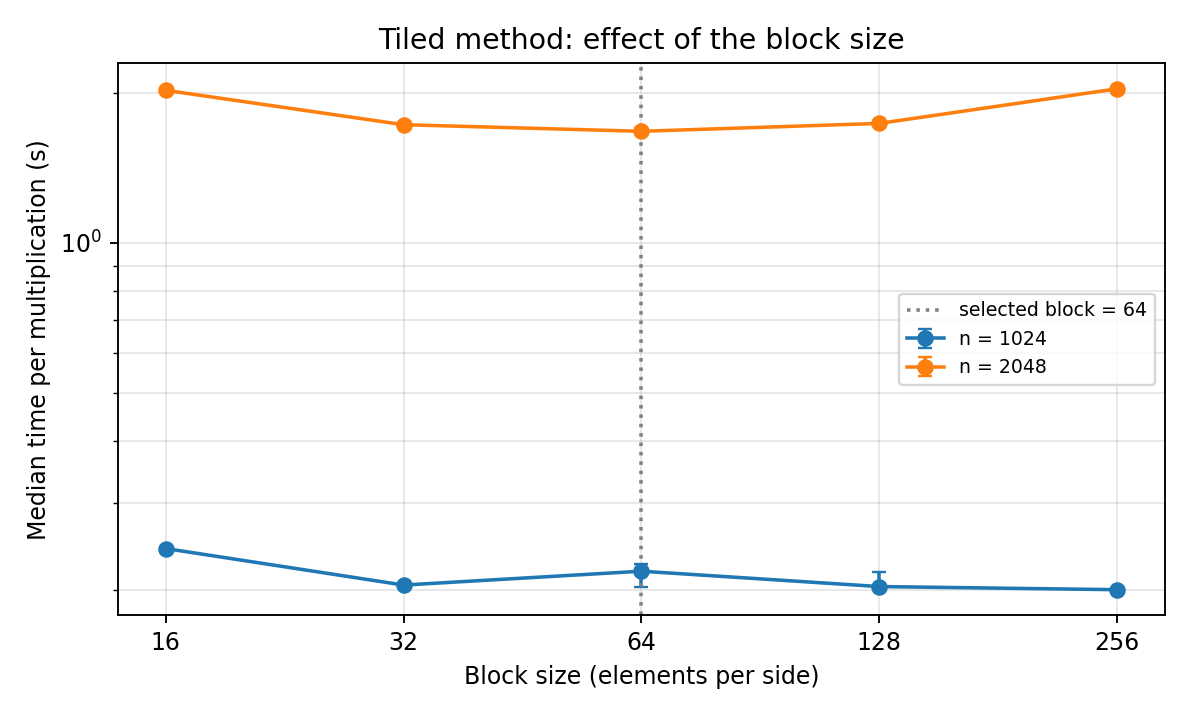
\includegraphics[width=0.75\textwidth]{fig1_block_tuning.png}
\caption{Tiled method: median time versus block size (bars: IQR).}
\label{fig:block}
\end{figure}

\section{Part A: dense methods}

\begin{table}[H]
\centering
\small
\caption{Dense methods: median time in seconds (IQR below 3\% of the median except where indicated) and speedup over
the baseline. All runs: 5 repetitions, except $n = 4096$ for \texttt{ikj} and \texttt{transpose} (3 repetitions).}
\label{tab:dense}
\resizebox{\textwidth}{!}{%
\begin{tabular}{r r rr rr rr}
\toprule
 & \textbf{naive} & \multicolumn{2}{c}{\textbf{ikj}} & \multicolumn{2}{c}{\textbf{transpose}} & \multicolumn{2}{c}{\textbf{tiled} ($b = 64$)} \\
\cmidrule(lr){2-2}\cmidrule(lr){3-4}\cmidrule(lr){5-6}\cmidrule(lr){7-8}
$n$ & time & time & speedup & time & speedup & time & speedup \\
\midrule
256  & 0.0117 & 0.00293 & 4.0 & 0.00587 & 2.0 & 0.00283 & 4.1 \\
512  & 0.111  & 0.0228 (IQR 4\%) & 4.9 & 0.0541  & 2.0 & 0.0236  & 4.7 \\
1000 & 0.502  & 0.183   & 2.7 & 0.427   & 1.2 & 0.166   & 3.0 \\
1024 & 2.140  & 0.196   & 10.9 & 0.502 (IQR 7\%) & 4.3 & 0.196 & 10.9 \\
2048 & 86.56  & 4.122   & 21.0 & 5.487   & 15.8 & 1.659 & 52.2 \\
4096 & timeout ($>$ 300 s) & 35.52 & -- & 44.63 & -- & 15.31 & -- \\
\bottomrule
\end{tabular}}
\end{table}

\begin{figure}[H]
\centering
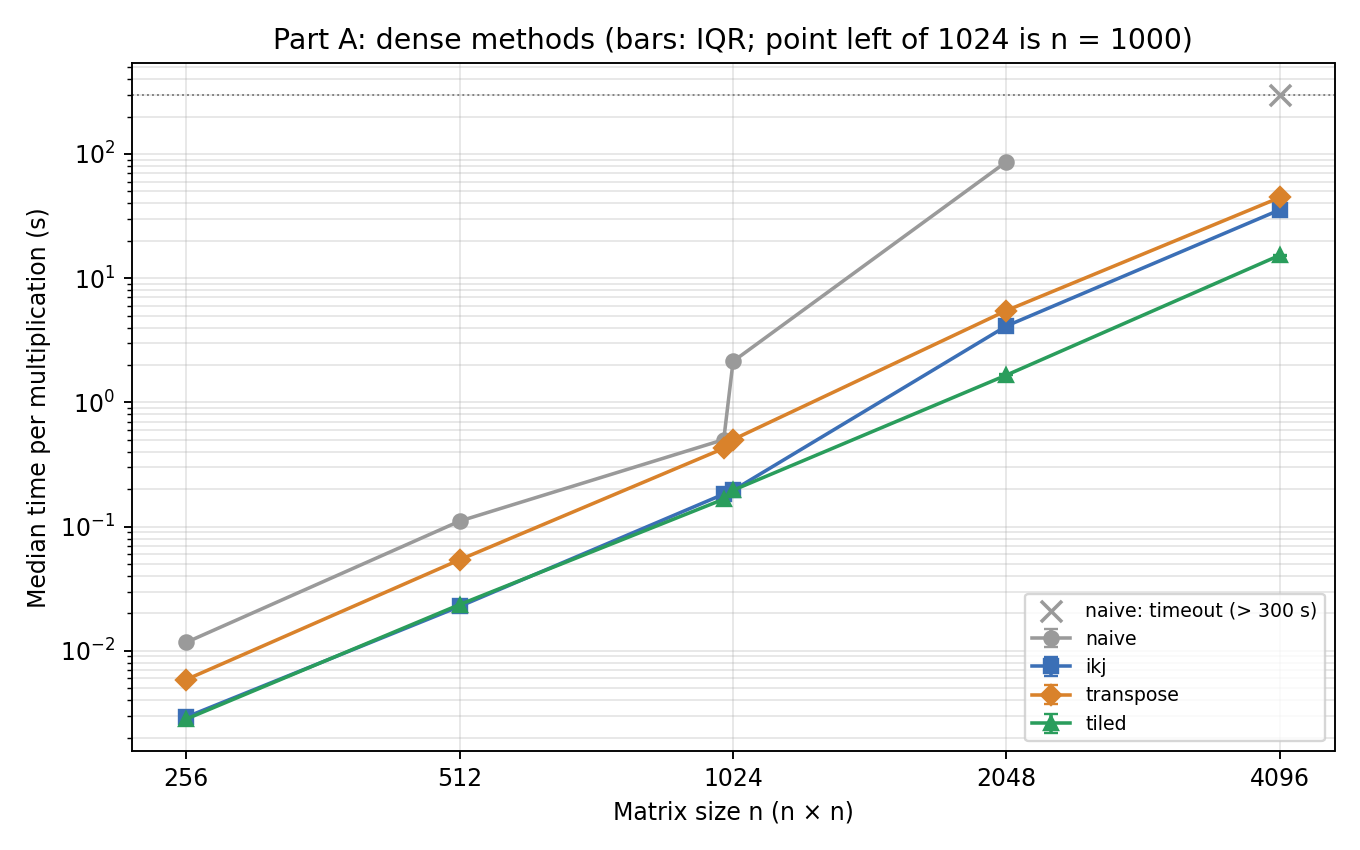
\includegraphics[width=0.85\textwidth]{fig2_dense_time.png}
\caption{Part A: median time versus $n$ (log--log; bars: IQR; the point just to the left of 1024 is $n = 1000$).}
\label{fig:densetime}
\end{figure}

\begin{figure}[H]
\centering
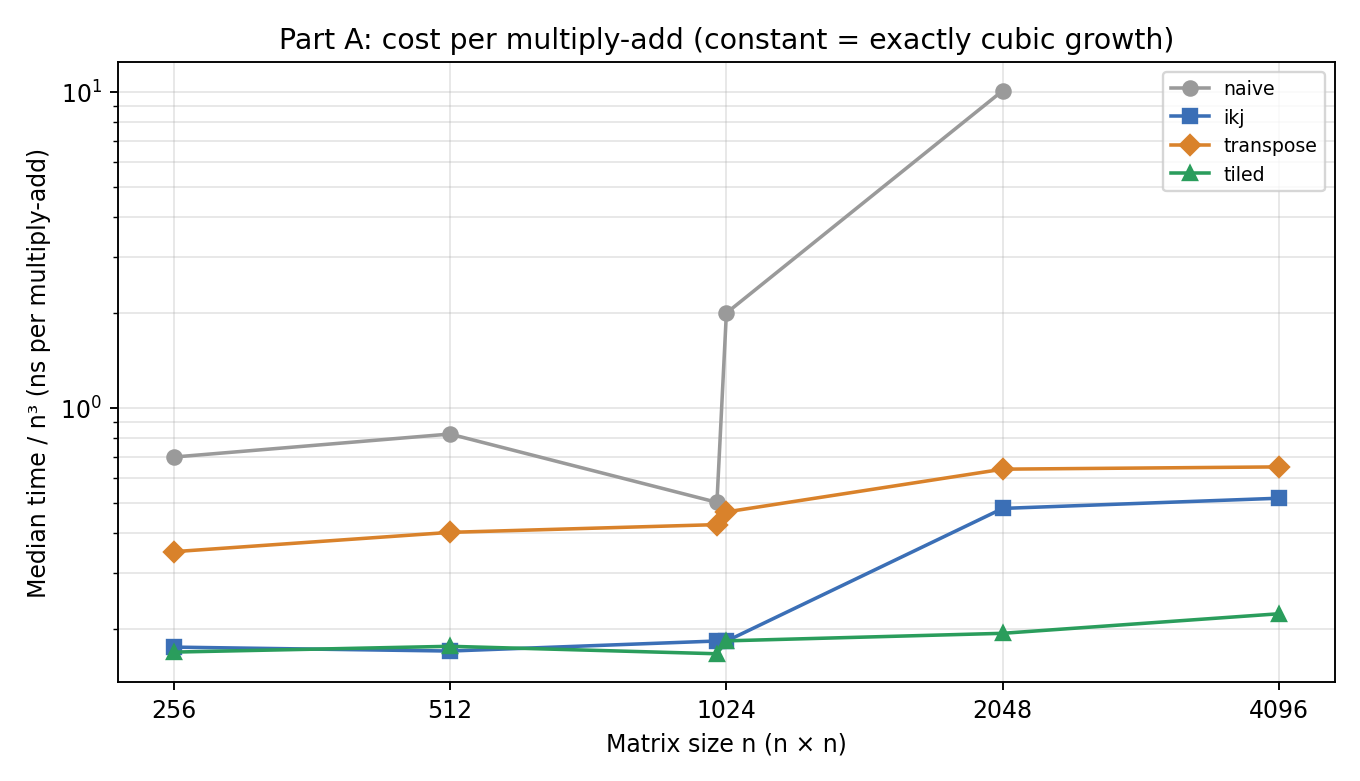
\includegraphics[width=0.85\textwidth]{fig3_dense_per_op.png}
\caption{Part A: median time divided by $n^3$. A horizontal line means exactly cubic growth.}
\label{fig:denseop}
\end{figure}

\begin{figure}[H]
\centering
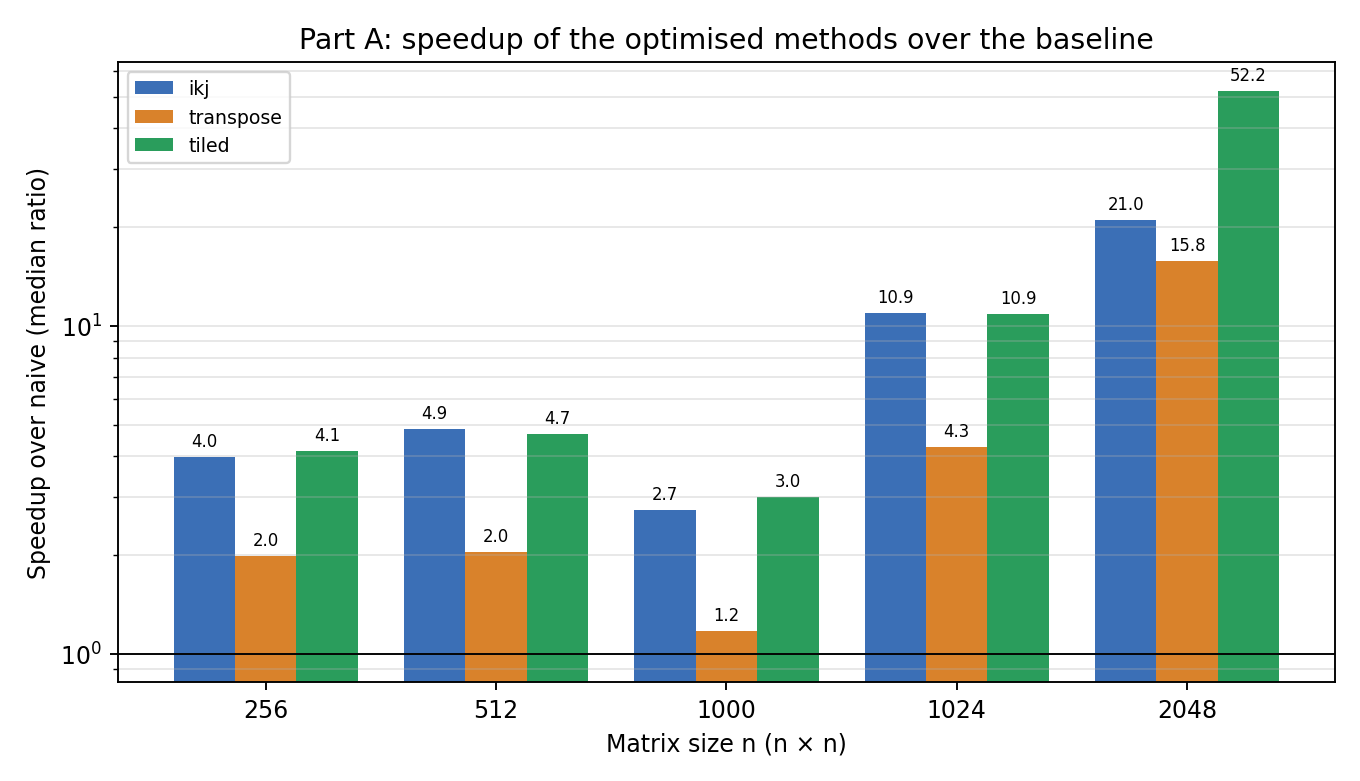
\includegraphics[width=0.85\textwidth]{fig4_dense_speedup.png}
\caption{Part A: speedup of each optimised method over the baseline (median ratio).}
\label{fig:speedup}
\end{figure}

\Cref{tab:dense} and \Cref{fig:densetime,fig:denseop,fig:speedup} show the main results. The cost per multiply-add of
the tiled method stays between 0.17 and 0.22~ns for all sizes, and its time grows by 9.2 from $n = 2048$ to $4096$
(cubic model: 8). The \texttt{ikj} method has the same cost as \texttt{tiled} up to $n = 1024$ (0.17--0.18~ns) but
rises to 0.48--0.52~ns for $n \geq 2048$. \texttt{transpose} costs 0.35--0.65~ns. The baseline goes from 0.70~ns at
$n = 256$ to 10.1~ns at $n = 2048$, and its time multiplies by 40 from $n = 1024$ to $2048$. Between $n = 1000$ and
$1024$ (cubic model: 1.07) the baseline becomes 4.3 times slower, \texttt{ikj} 1.07 times and \texttt{tiled} and
\texttt{transpose} 1.18 times. Peak memory is about $24n^2$ bytes for every method except \texttt{transpose}, which
needs the extra copy of $B^{\mathsf T}$ (516~MiB against 388~MiB for $n = 4096$).

\Cref{fig:freq} shows the effective clock of the pinned core, recorded every 0.5~s for configurations that lasted long
enough to be sampled. The optimised methods ran at 4.0--4.8~GHz, but the baseline ran at 3.1~GHz for $n = 2048$ and
1.7~GHz during the timed-out run with $n = 4096$, although all of them used the same core, power mode and
temperature conditions.

\begin{figure}[H]
\centering
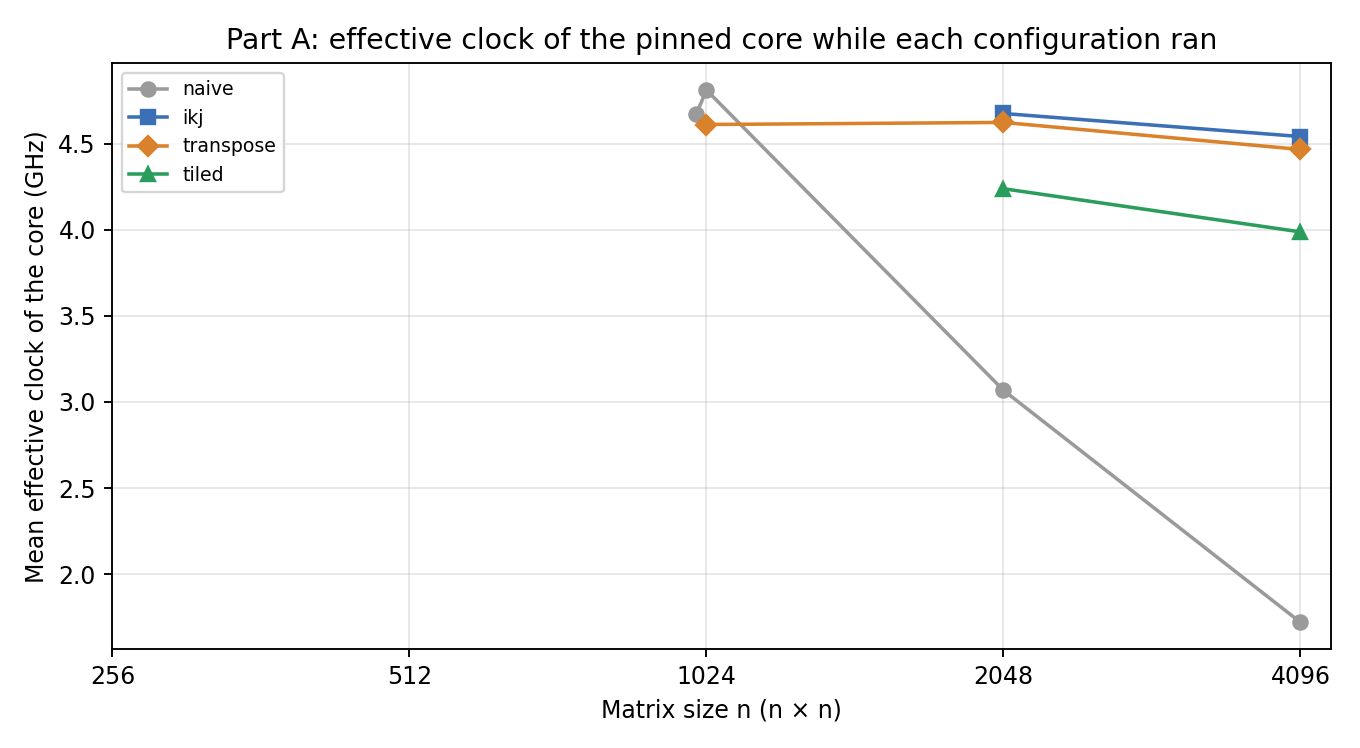
\includegraphics[width=0.8\textwidth]{fig8_core_frequency.png}
\caption{Part A: mean effective clock of the pinned core during each configuration (Windows counter
\textit{\% Processor Performance}; only configurations long enough to be sampled are shown).}
\label{fig:freq}
\end{figure}

\section{Part B: density and structure}

\begin{table}[H]
\centering
\small
\caption{Part B, $n = 2048$: nonzeros of each input and of the product, median times in seconds, and speedup of the
CSR product over the dense tiled product of the same matrices (without and with the conversion of $A$ and $B$).}
\label{tab:sparse}
\resizebox{\textwidth}{!}{%
\begin{tabular}{ll rrr rrr rr}
\toprule
 & & \multicolumn{3}{c}{\textbf{Nonzeros}} & \multicolumn{3}{c}{\textbf{Median time (s)}} & \multicolumn{2}{c}{\textbf{Speedup over dense}} \\
\cmidrule(lr){3-5}\cmidrule(lr){6-8}\cmidrule(lr){9-10}
Structure & $d$ (\%) & $\mathit{nnz}(A)$ & $\mathit{nnz}(C)$ & density $C$ (\%) & spgemm & dense & convert & spgemm & incl. conv. \\
\midrule
uniform & 0.01 & 419       & 75        & 0.002 & 0.0000308 & 1.622 & 0.0111 & 52\,660 & 146 \\
uniform & 0.1  & 4\,194    & 8\,661    & 0.21  & 0.000199  & 1.604 & 0.0117 & 8\,050  & 135 \\
uniform & 0.5  & 20\,972   & 209\,800  & 5.0   & 0.00882   & 1.623 & 0.0116 & 184     & 80 \\
uniform & 1    & 41\,943   & 777\,200  & 18.5  & 0.0393    & 1.611 & 0.0102 & 41      & 33 \\
uniform & 5    & 209\,715  & 4\,169\,000 & 99.4 & 0.279    & 1.637 & 0.0133 & 5.9     & 5.6 \\
uniform & 10   & 419\,430  & 4\,194\,304 & 100  & 0.307    & 1.634 & 0.0175 & 5.3     & 5.0 \\
uniform & 50   & 2\,097\,152 & 4\,194\,304 & 100 & 1.882   & 1.637 & 0.0448 & 0.87    & 0.85 \\
\addlinespace
banded & 0.01 & 419       & 87        & 0.002 & 0.0000351 & 1.552 & 0.0109 & 44\,220 & 143 \\
banded & 0.1  & 4\,194    & 6\,562    & 0.16  & 0.0000993 & 1.583 & 0.0111 & 15\,940 & 142 \\
banded & 0.5  & 20\,972   & 42\,290   & 1.0   & 0.000629  & 1.639 & 0.0121 & 2\,605  & 129 \\
banded & 1    & 41\,943   & 83\,380   & 2.0   & 0.00138   & 1.620 & 0.0120 & 1\,173  & 121 \\
banded & 5    & 209\,715  & 417\,000  & 9.9   & 0.0185    & 1.618 & 0.0123 & 87      & 52 \\
banded & 10   & 419\,430  & 817\,900  & 19.5  & 0.0585    & 1.610 & 0.0129 & 27.5    & 22.5 \\
banded & 50   & 2\,097\,152 & 3\,476\,000 & 82.9 & 1.282  & 1.623 & 0.0181 & 1.27    & 1.25 \\
\bottomrule
\end{tabular}}
\end{table}

\begin{figure}[H]
\centering
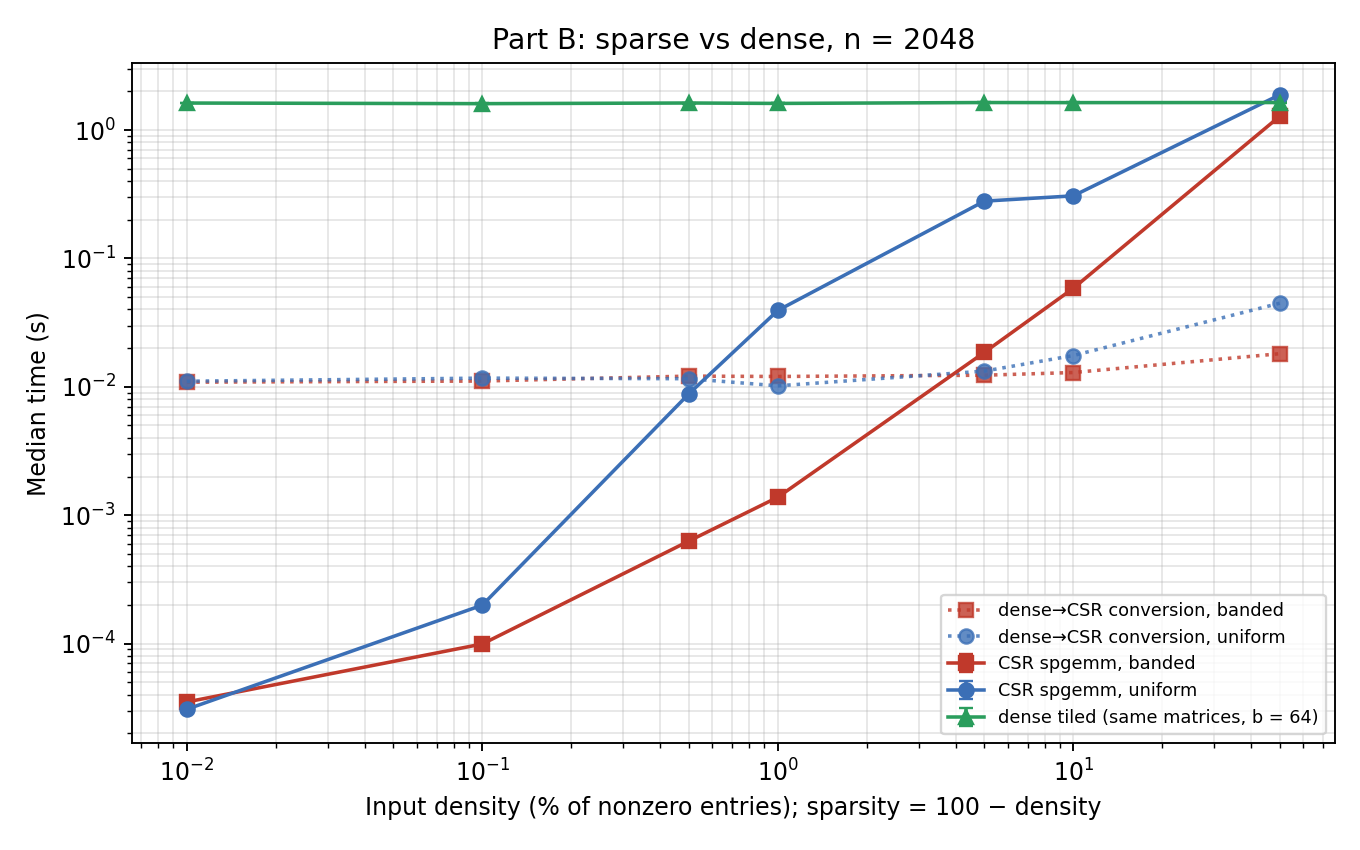
\includegraphics[width=0.85\textwidth]{fig5_sparse_density.png}
\caption{Part B, $n = 2048$: median time of the CSR product (solid), of the dense $\to$ CSR conversion (dotted) and of
the dense tiled product of the same matrices, versus input density.}
\label{fig:density}
\end{figure}

\begin{figure}[H]
\centering
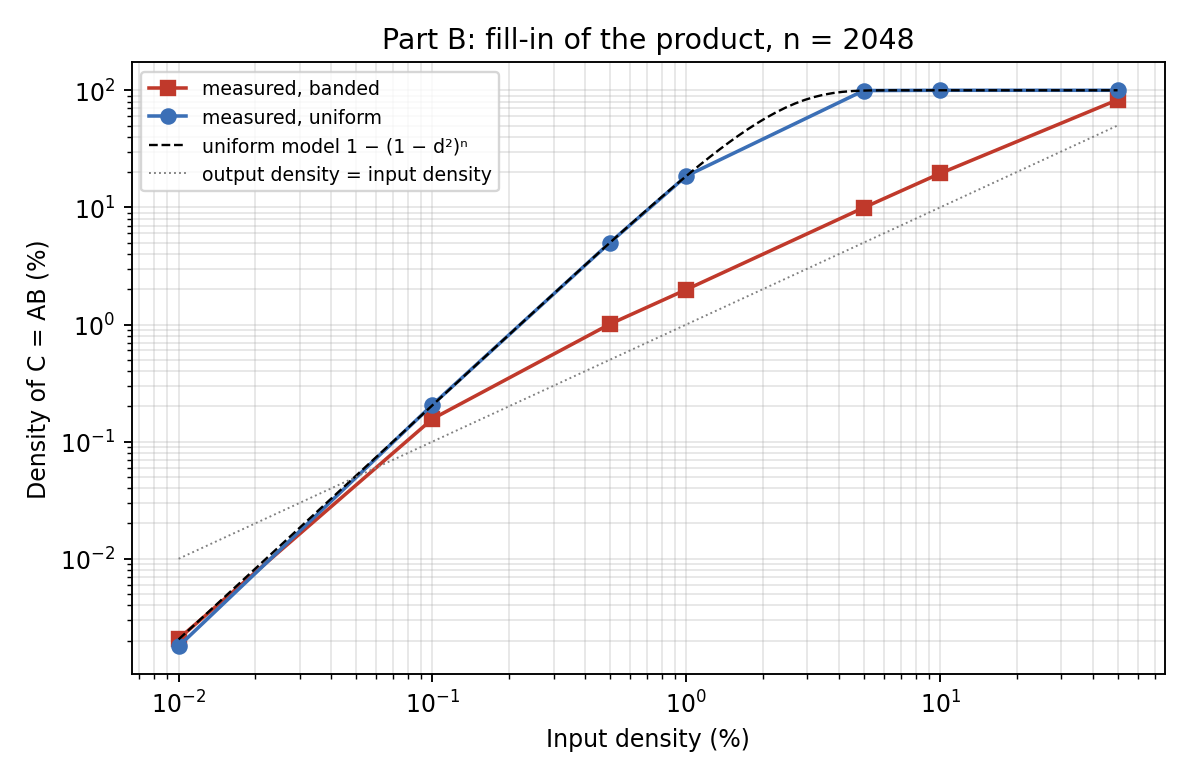
\includegraphics[width=0.75\textwidth]{fig6_fill_in.png}
\caption{Part B, $n = 2048$: density of the product versus density of the inputs, with the uniform model
$1 - (1 - d^2)^n$.}
\label{fig:fillin}
\end{figure}

The dense product takes 1.55--1.64~s for every input, independently of the number of zeros
(\Cref{tab:sparse}, \Cref{fig:density}). The CSR product is faster for every banded input and for uniform inputs up to
10\%, and slower for the uniform input with 50\%; interpolating in log--log scale, the break-even density for the
uniform structure is 44\% (43\% when the conversion is included), and no break-even exists in the tested range for the
banded structure. The conversion of $A$ and $B$ costs 10--45~ms, nearly independent of the density, which is more than
the CSR product itself for every density up to 0.5\% (uniform) or 1\% (banded).

\Cref{fig:fillin} shows that the measured density of the product of uniform matrices matches the model
$1 - (1 - d^2)^n$: it is 18.5\% for $d = 1\%$ and 99.4\% for $d = 5\%$. The product of banded matrices stays at about
twice the input density. With the same input density of 5\%, the uniform product has ten times more nonzeros and takes
15 times longer than the banded one. The cost per scalar multiply-add of the CSR product was 0.6--1.6~ns for banded
inputs with $d \geq 1\%$, but 13--46~ns for uniform inputs with $0.5\% \leq d \leq 5\%$; at the lowest densities it is
dominated by the per-row work and is not meaningful.

Peak memory was 4.5--18~MiB for the CSR product with $d \leq 1\%$ against 100~MiB for the dense product, but for uniform
inputs with $d \geq 5\%$ the CSR product needed 73--100~MiB, as much as the dense one, because the result is
practically dense and CSR needs 12~bytes per stored value instead of 8.

\section{Part B: size scaling}

\begin{table}[H]
\centering
\small
\caption{Part B, uniform structure with $d = 0.1\%$: median times (s), product density and peak memory (MiB).}
\label{tab:scaling}
\begin{tabular}{r rr rrr rr}
\toprule
$n$ & $\mathit{nnz}(A)$ & density $C$ (\%) & spgemm & dense & convert & mem.\ spgemm & mem.\ dense \\
\midrule
1024  & 1\,049      & 0.11 & 0.0000353 & 0.192 & 0.0022 & 4.4  & 28 \\
2048  & 4\,194      & 0.21 & 0.000208  & 1.594 & 0.0114 & 4.6  & 100 \\
4096  & 16\,777     & 0.41 & 0.00199   & 13.32 & 0.0480 & 5.7  & 388 \\
8192  & 67\,109     & 0.82 & 0.0211    & 110.2 & 0.195  & 12.2 & 1\,539 \\
16384 & 268\,435    & 1.63 & 0.209     & not run$^{*}$ & not run$^{*}$ & 60.8 & -- \\
32768 & 1\,073\,742 & 3.22 & 2.090     & not run$^{*}$ & not run$^{*}$ & 426  & -- \\
\bottomrule
\multicolumn{8}{l}{\footnotesize $^{*}$ Predicted array memory above the 4~GiB budget (dense: 6~GiB for $n = 16384$, 24~GiB for $n = 32768$).}
\end{tabular}
\end{table}

\begin{figure}[H]
\centering
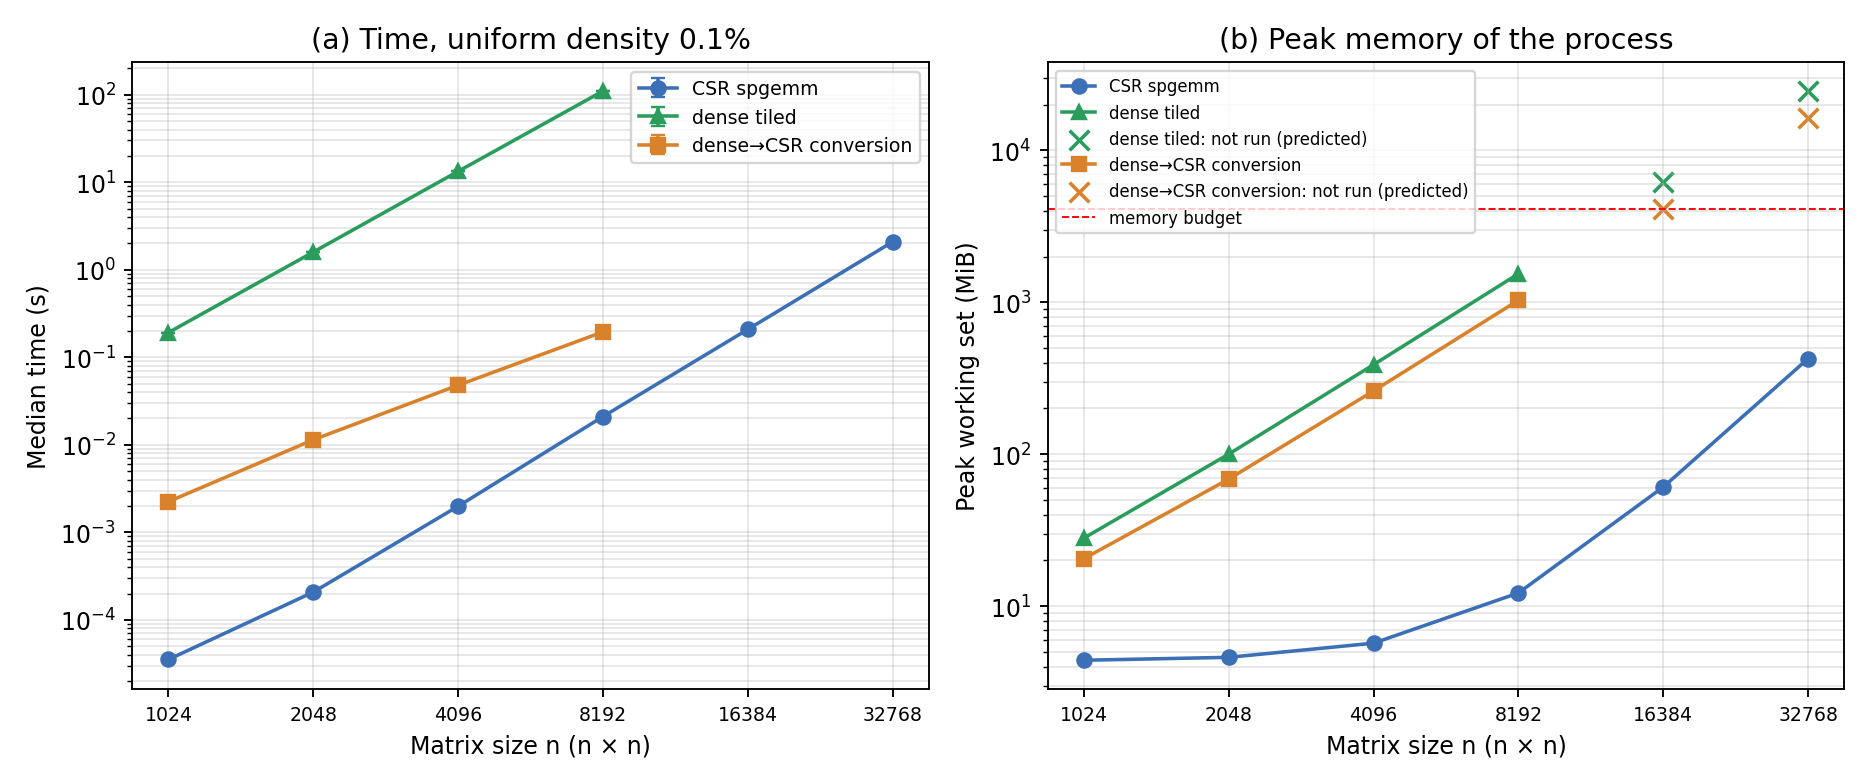
\includegraphics[width=\textwidth]{fig7_sparse_scaling.png}
\caption{Part B, uniform $d = 0.1\%$: (a) median time and (b) peak memory versus $n$. Crosses: predicted memory of
the configurations that were not run because they exceed the budget.}
\label{fig:scaling}
\end{figure}

For a fixed density of 0.1\%, the CSR product was 5\,200 to 7\,700 times faster than the dense product for
$n \leq 8192$ (\Cref{tab:scaling}, \Cref{fig:scaling}). Its time grows by about 10 per doubling of $n$ from
$n = 2048$ onwards (6 between 1024 and 2048), because both
the number of multiply-adds ($\propto d^2 n^3$) and the density of the product grow with $n$. The largest feasible
size was $n = 8192$ for the dense product and conversion, limited by memory, and $n = 32768$ (the largest tested) for
the CSR product.

% =================================================
\chapter{Discussion}
% =================================================

\section{Effect of the dense optimisations (H1--H3)}

\textbf{H1 is supported.} The three optimisations were faster than the baseline at every size, and the advantage grew
with $n$: from 2--4 times at $n = 256$ to 21 (\texttt{ikj}), 16 (\texttt{transpose}) and 52 (\texttt{tiled})
times at $n = 2048$. The only exception to the growth is $n = 1000$, where the baseline is not penalised by the
power-of-two effect and the gains are smaller (1.2--3.0 times). Because every method performs the same operations in
the same order and produces the same bits, these differences come only from the memory access pattern.

The cost per multiply-add explains the differences (\Cref{fig:denseop}). The innermost loop of \texttt{ikj} streams a
row of $B$ and a row of $C$; for $n \leq 1024$ all of $B$ (at most 8~MiB) fits in the 24~MB L3 cache, but for
$n = 2048$ it occupies 32~MiB, so every pass of the $k$ loop reads $B$ from main memory and the cost per operation
nearly triples. The tiled method works on $64 \times 64$ blocks (32~KiB each), so the block of $B$ being used stays in
the private caches and is reused for 64 rows of $C$; its cost per operation is almost independent of $n$, which is
exactly the behaviour expected from blocking~\cite{lam1991,goto2008}. \texttt{transpose} reads two contiguous rows,
but its inner loop is a reduction into a single accumulator, a chain of dependent additions that cannot be overlapped,
whereas the \texttt{ikj} and \texttt{tiled} inner loops update independent elements of $C$; this is a plausible reason
for its higher cost even when the data fits in cache, but it was not verified with hardware counters.

\textbf{H2 is supported.} \texttt{tiled} was the fastest method for $n \geq 2048$ and the only one whose cost per
operation stayed constant up to $n = 4096$, where it was 2.3 times faster than \texttt{ikj} and 2.9 times faster than
\texttt{transpose}. For $n \leq 1024$, where $B$ fits in the L3 cache, \texttt{ikj} and \texttt{tiled} were equivalent
(within 10\%, and within 1\% at $n = 1024$), so blocking only pays off once the working set exceeds the cache. The block size had a broad optimum
(32--128) on this processor; very small blocks add loop overhead and very large blocks no longer fit in the private
caches.

\textbf{H3 is supported.} The baseline was 4.3 times slower at $n = 1024$ than at $n = 1000$, as in
Assignment~1~\cite{a1}, because the column stride of a power-of-two matrix maps the elements of a column to few cache
sets. All the optimised methods avoid traversing columns, and their ratio between these two sizes is 1.07--1.18,
close to the cubic prediction of 1.07.

\paragraph{Clock frequency and the baseline.} The baseline at $n = 2048$ ran at 3.1~GHz and the optimised methods at
4.0--4.8~GHz on the same core (\Cref{fig:freq}). The power management of the processor lowered the clock when the core
was mostly stalled waiting for memory, which is the situation of the column-wise traversal of the baseline. Part of
the 52-times speedup of \texttt{tiled} at $n = 2048$ is therefore a frequency effect; scaling the baseline time by the
ratio of the clocks (3.07/4.24) still leaves a speedup of about 38. The same baseline code and inputs took 32.2~s in
Assignment~1 (14 October 2026) and 86.6~s in this study; running the unmodified Assignment~1 binary on the same day as
this study also took 93~s, so the difference is not due to the code. Windows and Intel graphics driver updates were
installed between the two dates, but the exact cause could not be identified. For this reason absolute times should
only be compared within the same study; all comparisons in this report were measured in a single run under the same
conditions.

\section{When does the sparse representation pay off? (H4--H5)}

\textbf{H4 is supported, and it shows that density alone does not determine the performance.} The dense product does
not benefit from zeros, so its time is constant, while the CSR product's work depends on the number of useful
multiply-adds and on the size of the result. For uniform matrices both grow very fast: the result is 99\% dense from
$d = 5\%$, so above that point the CSR product produces a dense matrix through a slower, indirect path, and its
advantage vanishes at about 44\%. Banded matrices with the same density produce only twice as many nonzeros, their
rows of $B$ are close to each other, and the touched columns of the accumulator form a narrow range, which explains
their much lower cost per operation (0.6--1.6~ns against 13--46~ns) and why the CSR product was still faster at 50\%.
With the same 5\% density, the uniform product was 15 times slower than the banded one. The break-even density
depends on $n$ as well, because the fill-in grows with $d^2 n$.

The conversion from dense to CSR costs $O(n^2)$ regardless of the density (10--45~ms for $n = 2048$). It does not
change the break-even density, but for very sparse inputs it dominates: the speedup over the dense product falls from
more than 40\,000 to about 140 when the conversion is included. In practice, sparse data should be generated or read
directly in a sparse format rather than converted from a dense array.

\textbf{H5 is supported.} At $d = 0.1\%$ the dense product needs $24n^2$ bytes and was limited to $n = 8192$ by the
4~GiB budget (1.5~GiB and 110~s), while the CSR product handled $n = 32768$ in 2.1~s and 426~MiB. The advantage is not
unlimited: the density of the product grew from 0.1\% to 3.2\% over this range, so for even larger $n$ at the same
input density the result would eventually become dense.

\section{Optimisation versus sparse storage}

The two parts improve performance by different mechanisms. The dense optimisations do not change the amount of
arithmetic: they reduce the cost of each operation, at most by a factor of about 50 here, and their benefit grows with
$n$. Sparse storage reduces the amount of work and memory, and its benefit can be several orders of magnitude, but only
while the inputs and the result stay sparse; it depends on the density, on the structure of the nonzeros, on $n$ and
on the conversion costs, and it can be slower than a good dense method for dense results.

\section{Limitations}

\begin{itemize}
  \item All measurements come from one laptop and one core; no hardware performance counters (cache, TLB misses) were
  collected, so the explanations based on the memory hierarchy are inferred from the timing patterns and from the
  clock measurements.
  \item The power management of the processor changes the clock during memory-bound phases. The clock was recorded,
  but not fixed, so the comparison with the baseline mixes memory effects and frequency effects.
  \item The absolute times of the baseline changed between Assignment~1 and this study for reasons that could not be
  identified (see above).
  \item Only one sparse format (CSR), one algorithm (Gustavson with a dense accumulator) and two synthetic structures
  were tested; real sparse matrices have other structures. No optimised sparse library was benchmarked.
  \item Only one size ($n = 2048$) was used for the density sweep, and only uniform matrices with $d = 0.1\%$ for the
  scaling study.
  \item The blocked method uses a single level of blocking with square blocks and no vectorisation; optimised BLAS
  libraries use several levels and are much faster~\cite{goto2008}.
\end{itemize}

% =================================================
\chapter{Conclusions}
% =================================================

Within the tested implementations, inputs and machine, this study establishes that:
\begin{itemize}
  \item Changing only the order of the same operations makes the dense multiplication up to 52 times faster
  ($n = 2048$). Cache blocking with blocks of 32--128 elements is the most effective technique for large matrices: its
  cost per operation stays almost constant up to $n = 4096$, so it follows the cubic model, while loop reordering
  degrades once a matrix no longer fits in the L3 cache.
  \item The optimisations remove the power-of-two penalty of the baseline.
  \item Memory-bound code can also lower the clock frequency chosen by the processor, which amplifies the cost of a
  poor access pattern.
  \item A CSR product is faster than a dense product of the same matrices below a break-even density of about 44\% for
  uniformly random nonzeros at $n = 2048$, and in the whole tested range for banded nonzeros. The difference is caused
  by fill-in: uniform sparse matrices produce dense results quickly. Density alone does not determine the result.
  \item The conversion from dense to CSR costs $O(n^2)$ and dominates for very sparse inputs.
  \item For very sparse matrices, sparse storage makes much larger problems feasible: at 0.1\% density, $n = 32768$
  took 2.1~s and 426~MiB, while the dense product was limited to $n = 8192$ by memory.
\end{itemize}
Open questions for future work are the direct measurement of cache misses and clock behaviour, other sparse formats and
real matrices, and the combination of these techniques with the parallel execution of Assignment~3.

% =================================================
\chapter*{AI Usage Statement}
\addcontentsline{toc}{chapter}{AI Usage Statement}
% =================================================

In accordance with the course policy, a generative AI assistant was used to support the planning of the experiments,
the development and debugging of the benchmark code and scripts, and the language revision of this report. All the
measurements were executed on the author's computer, and the author checked the code, the results and the references
and is responsible for the conclusions.

% =================================================
\chapter*{Reproducibility Materials}
\addcontentsline{toc}{chapter}{Reproducibility Materials}
% =================================================

All materials are in the folder \texttt{assignment2} of the repository
\url{https://github.com/Claudia1771/bigdata-matrix-multiplication}:
\begin{itemize}
  \item \texttt{src/dense.c} and \texttt{src/sparse.c}: the implementations (the baseline is the code of
  \texttt{assignment1}).
  \item \texttt{config.json}: seeds, sizes, densities, structures, repetitions, budgets, flags and CPU affinity.
  \item \texttt{scripts/}: \texttt{generate\_inputs.py}, \texttt{verify.py}, \texttt{run\_experiment.py},
  \texttt{analyze.py} and \texttt{common.py}.
  \item \texttt{results/}: \texttt{inputs\_manifest.csv} (seeds and SHA-256 hashes), \texttt{correctness.csv}, raw
  measurements, run conditions, summaries, figures, and the two discarded runs.
  \item \texttt{README.md}: exact build and run commands and dependency versions.
\end{itemize}

% =================================================
% REFERENCES
% =================================================
\begin{thebibliography}{99}
\addcontentsline{toc}{chapter}{References}

\bibitem{a1} C.~Álvarez González, ``How matrix size affects runtime and memory of a basic triple-loop matrix
multiplication in Python, Java and C,'' Big Data, Individual Assignment~1, Univ. Las Palmas de Gran Canaria, Oct.~2026.
[Online]. Available: \url{https://github.com/Claudia1771/bigdata-matrix-multiplication}

\bibitem{gustavson1978} F.~G. Gustavson, ``Two fast algorithms for sparse matrices: Multiplication and permuted
transposition,'' \textit{ACM Trans. Math. Softw.}, vol.~4, no.~3, pp.~250--269, 1978.

\bibitem{saad2003} Y.~Saad, \textit{Iterative Methods for Sparse Linear Systems}, 2nd~ed. Philadelphia, PA, USA:
SIAM, 2003.

\bibitem{davis2006} T.~A. Davis, \textit{Direct Methods for Sparse Linear Systems}. Philadelphia, PA, USA: SIAM, 2006.

\bibitem{lam1991} M.~S. Lam, E.~E. Rothberg, and M.~E. Wolf, ``The cache performance and optimizations of blocked
algorithms,'' in \textit{Proc. 4th Int. Conf. Architectural Support for Programming Languages and Operating Systems
(ASPLOS-IV)}, 1991, pp.~63--74.

\bibitem{goto2008} K.~Goto and R.~A. van~de~Geijn, ``Anatomy of high-performance matrix multiplication,''
\textit{ACM Trans. Math. Softw.}, vol.~34, no.~3, Art.~no.~12, 2008.

\bibitem{leiserson2020} C.~E. Leiserson, N.~C. Thompson, J.~S. Emer, B.~C. Kuszmaul, B.~W. Lampson, D.~Sanchez, and
T.~B. Schardl, ``There's plenty of room at the Top: What will drive computer performance after Moore's law?,''
\textit{Science}, vol.~368, no.~6495, Art.~no.~eaam9744, 2020.

\bibitem{drepper2007} U.~Drepper, ``What every programmer should know about memory,'' Red Hat, Inc., Tech. Rep.,
Nov.~2007.

\bibitem{hoefler2015} T.~Hoefler and R.~Belli, ``Scientific benchmarking of parallel computing systems: Twelve ways to
tell the masses when reporting performance results,'' in \textit{Proc. Int. Conf. High Performance Computing,
Networking, Storage and Analysis (SC15)}, 2015, Art.~no.~73.

\end{thebibliography}

\end{document}
